\chapter{Optimierung des ARM-Codes}
\label{ch:optarm}
\rm

In diesem Kapitel sollen die Anfangsbedingungen, die Ansatzpunkte, die Konzepte der durchgef�hrten Optimierungen am ARM-Code des \textit{Music Classificators} vorgestellt werden.\\
Hierzu sollen in \textbf{Kapitel \ref{sec:fset}} zuerst die Featuresets vorgestellt werden, welche f�r die Messungen der Laufzeit des Programms verwendet wurden, aus denen in \textbf{Kapitel \ref{sec:ansatz}} die wesentlichen
Bottlenecks und Optimierungspotenziale auf dem DaVinci\texttrademark extrahiert werden sollen. \textbf{Kapitel \ref{sec:optFFT}} befasst sich daraufhin den Konzepten und der Durchf�hrung von Optimierungen der FFT.

\section{Featuresets}\label{sec:fset}

F�r die Laufzeitanalysen des \textit{Music Classificators} wurden vier verschiedene Featuresets (im sp�teren mit \textit{FSetN} bezeichnet) verwendet, die in den folgenden Unterkapiteln n�her spezifiziert werden sollen. Diese Featuresets wurden nicht selbst erstellt, sondern so aus der Literatur �bernommen. Die einzelnen Referenzen sind passen zu den Featuresets angegeben.

\subsection{Featureset 1 (FSet1)}\label{subsec:fset1}

\begin{itemize}
	\item Spectral Centroid (\textbf{\ref{subsubsec:sc}})
	\item Spectral Rolloff (\textbf{\ref{subsubsec:sr}})
	\item Spectral Flux (\textbf{\ref{subsubsec:sf}})
	\item MFCC (\textbf{\ref{subsubsec:mfcc}})
\end{itemize}

\subsection{Featureset 2 (FSet2)}\label{subsec:fset2}

\begin{itemize}
	\item Normalized Audio Spectrum Envelope (\textbf{\ref{subsubsec:nase}})
	\item Octave Spectral Contrast (\textbf{\ref{subsubsec:osc}})
	\item MFCC (\textbf{\ref{subsubsec:mfcc}})
\end{itemize}

\subsection{Featureset 3 (FSet3)}\label{subsec:fset3}

\begin{itemize}
	\item Low Energy (\textbf{\ref{subsubsec:le}})
	\item Root Mean Square (\textbf{\ref{subsubsec:rms}})
	\item Zero Crossing Rate (\textbf{\ref{subsubsec:zcr}})
\end{itemize}

\subsection{Featureset 4 (FSet4)}\label{subsec:fset4}

\begin{itemize}
	\item Ampitude of Maximum In Chromagram (\textbf{\ref{subsubsec:aomic}})
	\item Specral Crest Factor (\textbf{\ref{subsubsec:scf}})
	\item Sub-Band Energy Ratio (\textbf{\ref{subsubsec:sber}})
\end{itemize}

\section{Ansatzpunkte und Bottlenecks}\label{sec:ansatz}

Auf Basis der in \textbf{Kapitel \ref{sec:fset}} vorgestellten Featuresets sollen nun die vor Beginn der Optimierung durchgef�hrten Laufzeitmessungen vorgestellt und er�rtert werden. Es wurden zwei unterschiedliche Messreihen durchgef�hrt, die sich in den gew�hlten Optimierungen unterscheiden, die vom Compiler zur Compilezeit automatisch durchgef�hrt werden k�nnen. F�r die erste Messreihe wurde lediglich der Compilerflag \textit{-O3} verwendet, welches f�r die h�chste automatische Compileroptimierung steht, diese Messreihe soll f�r weitere Betrachtungen als \textit{Unoptimized} bezeichnet werden. \\
Die zweite Messreihe schlie�t die in \textbf{Kapitel \ref{subsec:neon}} vorgestellte NEON-Einheit ein. Auch f�r diese Messreihe wurden keine NEON-spezifischen Optimierungen des Codes vorgenommen, sondern nur die vom Compiler angebotene Option aktiviert, den Code w�hrend des Compilings selber f�r den NEON zu optimieren, im Weiteren wird diese Messreihe als \textit{NEON Autocompiler} bezeichnet. \\
Die Laufzeitanteile der drei Programmteile \textit{Extraction}, \textit{Processing} und \textit{Classification} sind in \textbf{Abbildung \ref{fig:ResultsMCL}} dargestellt.\\

\begin{figure}[ht]
	\centering
		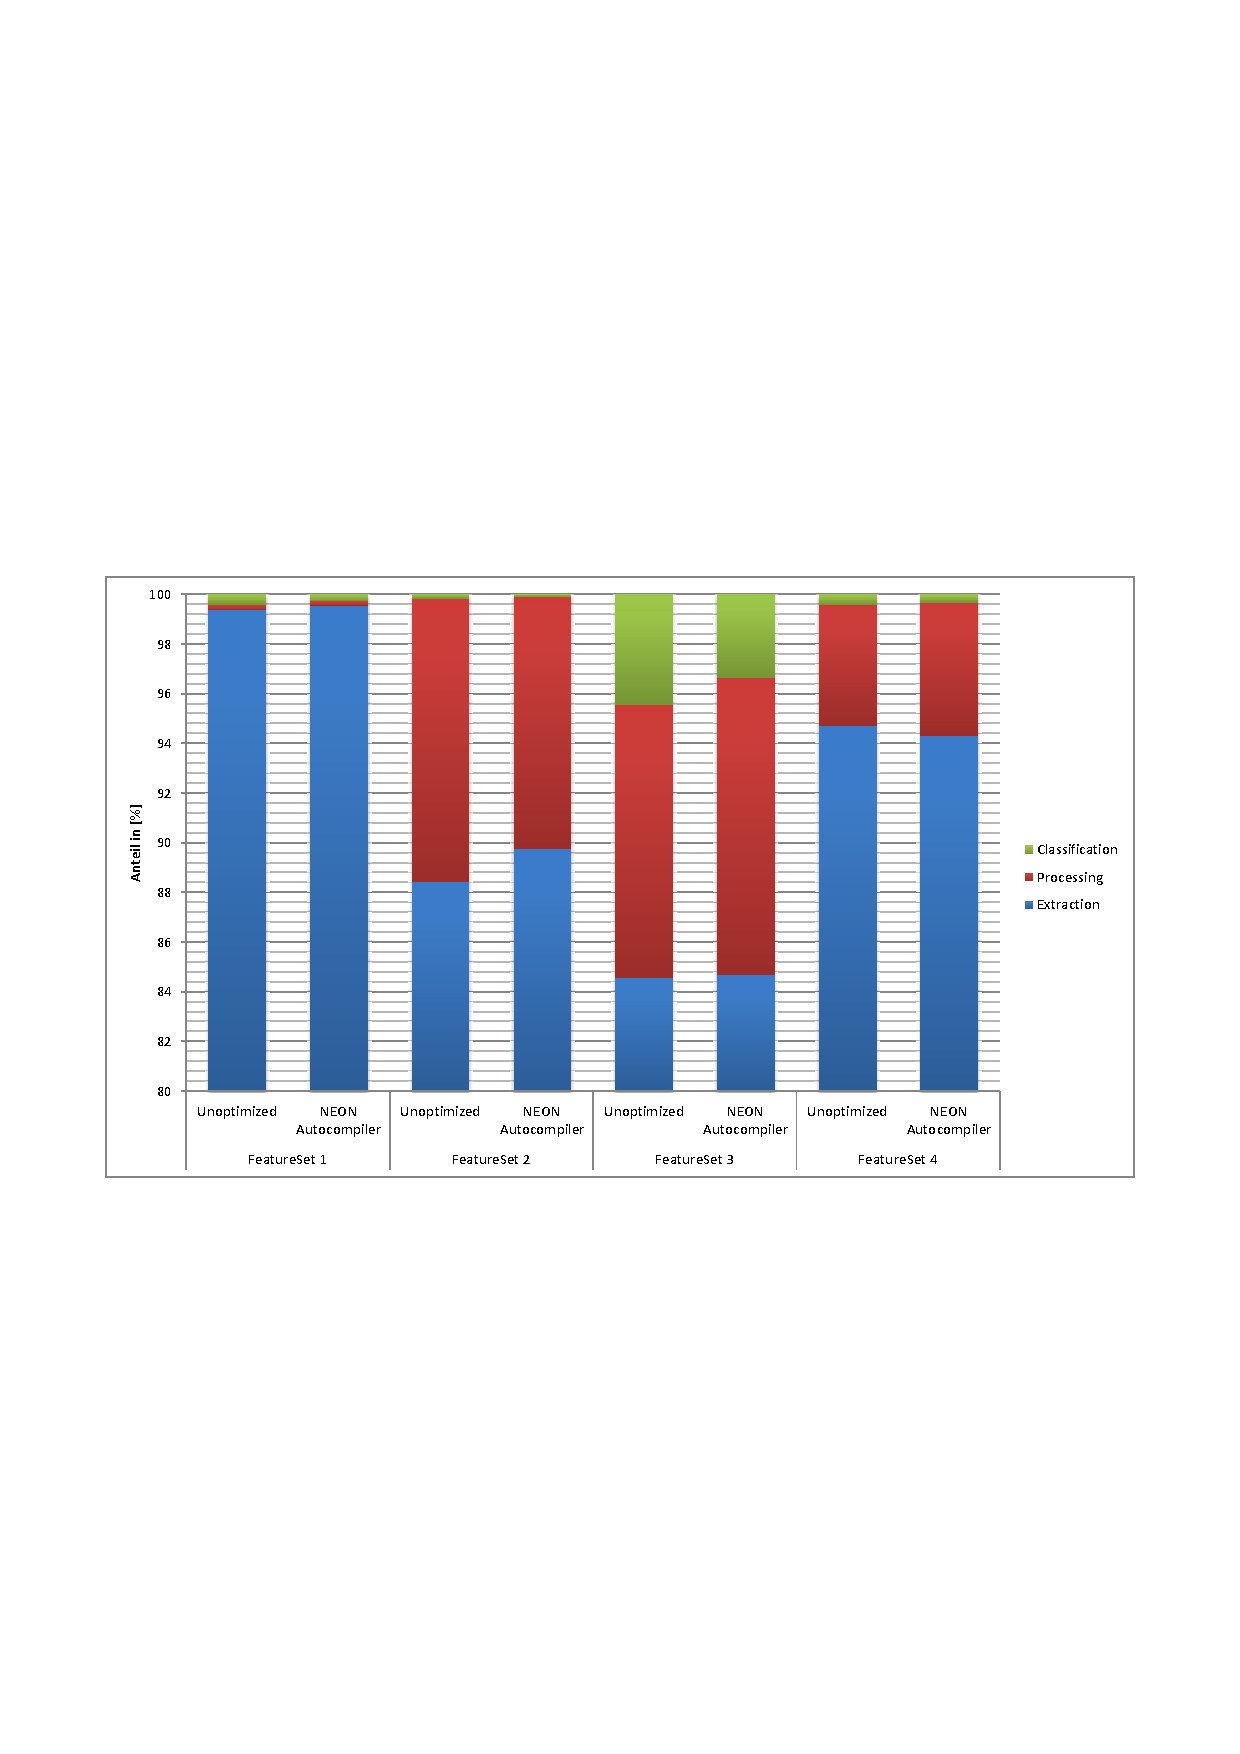
\includegraphics[width=1.00\textwidth]{../Pictures/ResultsMCL.pdf}
	\caption{Laufzeitanteile ohne manuelle Optimierung}
	\label{fig:ResultsMCL}
\end{figure}

Wie man leicht erkennen kann hat die Extraktion bei allen vier Featuresets mit teilweise weit �ber 80\% den gr��ten Anteil an der Laufzeit des Programms, daher wird im Nachfolgenden die Extraktion noch etwas detailierter betrachtet werden. \\
\textbf{Abbildung \ref{fig:ResultsExtraction}} zeigt die Anteile der einzelnen Features an der Gesammtlaufzeit der Extraktion. Hier soll daran erinnert werden, dass \textit{FSet1}, \textit{FSet2} und \textit{FSet4} aus Features bestehen, die aus dem Frequenzbereich stammen, wodurch vor der Extraktion erst eine Fourier-Transformation vom Zeitbereich in diesen stattfinden muss, weshalb als weiteres "`Feature"' die FFT in der Abbildung auftaucht. Desweiteren arbeitet das Feature \textit{Ampitude of Maximum In Chromagram}aus \textit{FSet4} auf dem in \textbf{Kapitel \ref{subsubsec:cv}} vorgestellten \textit{Chroma Vector}, was dazuf�hrt, dass auch dieser in der Abbildung auftaucht.

\begin{figure}[ht]
	\centering
		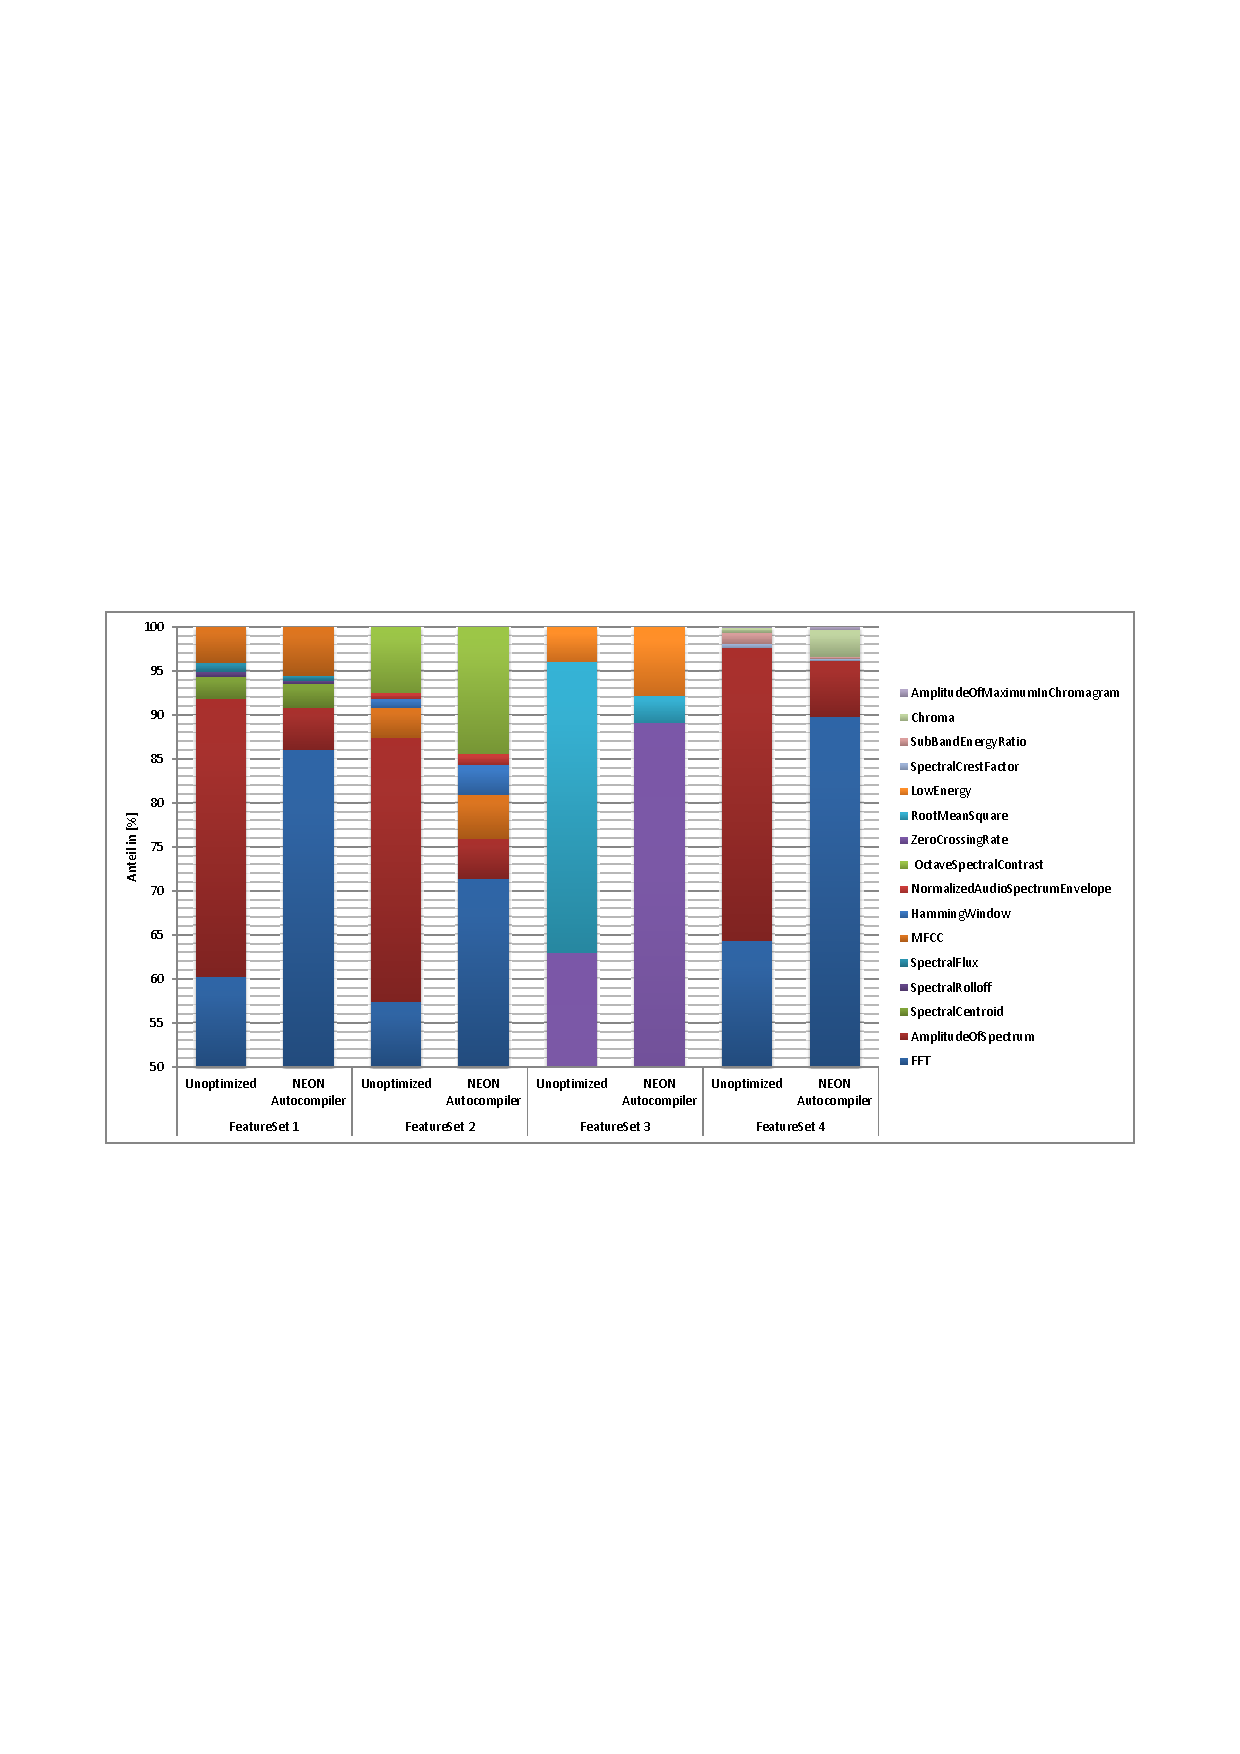
\includegraphics[width=1.00\textwidth]{../Pictures/ResultsExtraktion.pdf}
	\caption{Detailierte Laufzeitenanteile der Extraktion ohne manuelle Optimierung}
	\label{fig:ResultsExtraction}
\end{figure}

Wie man der \textbf{Abbildung \ref{fig:ResultsExtraction}} entnehmen kann, hat gerade diese Transformation vom Zeit- in den Frequenzbereich den gr��ten Laufzeitbedarf, ihr Anteil liegt immer �ber 50\%. Um Irritationen zu vermeiden, soll darauf hingewiesen werden, dass sich die Laufzeit der FFT in \textit{NEON Autocompiler} nicht, wie es in der Abbildung den Anschein hat, drastisch verschlechtert hat, sondern die Verbesserungen der tats�chlichen Feature-Extraktionen sich dahingehend verbessert haben, dass die \textit{FFT} dadurch einen prozentual gr��eren Anteil einnimmt. Um genauer zu sein, hat sich in den Experimenten gezeigt, dass sich die Laufzeit der \textit{FFT} in nahezu allen F�llen fast halbiert hat.\\
Da sich gezeigt hat, dass die \textit{FFT} den gr��ten Anteil an der Laufzeit hat und das diese durch die NEON-Einheit vom Compiler schon gut optimiert werden konnte, soll im n�chsten Kapitel betrachtet werden, ob dieses durch gezielte Optimierungen bez�glich der NEON-Einheit im Code noch weiter verbessert werden kann.


\section{Optimierung der FFT}\label{sec:optFFT}
Wie im vorherigen Abschnitt gezeigt wurde, nimmt die Berechnung der \textit{FFT} die gr��ten Anteil an der Laufzeit ein. Au�erdem wurde gezeigt, dass diese ein gutes Optimierungspotenzial hinsichtlich der NEON-Einheit besitzt. Da eine NEON-Optimierung des FFT-Codes viel Zeit in Anspruch nehmen k�nnte und bereits FFT-Bibliotheken verf�gbar sind, die hinsichtlich der NEON-Einheit optimiert wurden.\\
Im Nachfolgenden sollen daher die FFT-Bibliotheken \textit{"`Fastest Fourier Transformation in the West"'} (\textbf{\ref{subsec:fftw}}), \textit{"`Fastest Fourier Transformation in the South"'} (\textbf{\ref{subsec:ffts}}), \textit{"`Cricket FFT"'} (\textbf{\ref{subsec:cfft}}) und \textit{"`Libav"'} (\textbf{\ref{subsec:libav}}) vorgestellt und in \textbf{Abbschnitt \ref{subsec:rfft}} anhand ihrer Laufzeitverbesserungen verglichen werden.

\subsection{Fastest Fourier Transformation in the West (FFTW)}\label{subsec:fftw}

\subsection{Fastest Fourier Transformation in the South (FFTS}\label{subsec:ffts}

\subsection{Criket FFT}\label{subsec:cfft}

\subsection{Libav}\label{subsec:libav}

\subsection{Laufzeitvergleich der FFTs}\label{subsec:rfft}

 